% Options for packages loaded elsewhere
\PassOptionsToPackage{unicode}{hyperref}
\PassOptionsToPackage{hyphens}{url}
%
\documentclass[
  ,pub,floatsintext]{apa6}
\usepackage{amsmath,amssymb}
\usepackage{lmodern}
\usepackage{iftex}
\ifPDFTeX
  \usepackage[T1]{fontenc}
  \usepackage[utf8]{inputenc}
  \usepackage{textcomp} % provide euro and other symbols
\else % if luatex or xetex
  \usepackage{unicode-math}
  \defaultfontfeatures{Scale=MatchLowercase}
  \defaultfontfeatures[\rmfamily]{Ligatures=TeX,Scale=1}
\fi
% Use upquote if available, for straight quotes in verbatim environments
\IfFileExists{upquote.sty}{\usepackage{upquote}}{}
\IfFileExists{microtype.sty}{% use microtype if available
  \usepackage[]{microtype}
  \UseMicrotypeSet[protrusion]{basicmath} % disable protrusion for tt fonts
}{}
\makeatletter
\@ifundefined{KOMAClassName}{% if non-KOMA class
  \IfFileExists{parskip.sty}{%
    \usepackage{parskip}
  }{% else
    \setlength{\parindent}{0pt}
    \setlength{\parskip}{6pt plus 2pt minus 1pt}}
}{% if KOMA class
  \KOMAoptions{parskip=half}}
\makeatother
\usepackage{xcolor}
\usepackage{graphicx}
\makeatletter
\def\maxwidth{\ifdim\Gin@nat@width>\linewidth\linewidth\else\Gin@nat@width\fi}
\def\maxheight{\ifdim\Gin@nat@height>\textheight\textheight\else\Gin@nat@height\fi}
\makeatother
% Scale images if necessary, so that they will not overflow the page
% margins by default, and it is still possible to overwrite the defaults
% using explicit options in \includegraphics[width, height, ...]{}
\setkeys{Gin}{width=\maxwidth,height=\maxheight,keepaspectratio}
% Set default figure placement to htbp
\makeatletter
\def\fps@figure{htbp}
\makeatother
\setlength{\emergencystretch}{3em} % prevent overfull lines
\providecommand{\tightlist}{%
  \setlength{\itemsep}{0pt}\setlength{\parskip}{0pt}}
\setcounter{secnumdepth}{-\maxdimen} % remove section numbering
% Make \paragraph and \subparagraph free-standing
\ifx\paragraph\undefined\else
  \let\oldparagraph\paragraph
  \renewcommand{\paragraph}[1]{\oldparagraph{#1}\mbox{}}
\fi
\ifx\subparagraph\undefined\else
  \let\oldsubparagraph\subparagraph
  \renewcommand{\subparagraph}[1]{\oldsubparagraph{#1}\mbox{}}
\fi
\newlength{\cslhangindent}
\setlength{\cslhangindent}{1.5em}
\newlength{\csllabelwidth}
\setlength{\csllabelwidth}{3em}
\newlength{\cslentryspacingunit} % times entry-spacing
\setlength{\cslentryspacingunit}{\parskip}
\newenvironment{CSLReferences}[2] % #1 hanging-ident, #2 entry spacing
 {% don't indent paragraphs
  \setlength{\parindent}{0pt}
  % turn on hanging indent if param 1 is 1
  \ifodd #1
  \let\oldpar\par
  \def\par{\hangindent=\cslhangindent\oldpar}
  \fi
  % set entry spacing
  \setlength{\parskip}{#2\cslentryspacingunit}
 }%
 {}
\usepackage{calc}
\newcommand{\CSLBlock}[1]{#1\hfill\break}
\newcommand{\CSLLeftMargin}[1]{\parbox[t]{\csllabelwidth}{#1}}
\newcommand{\CSLRightInline}[1]{\parbox[t]{\linewidth - \csllabelwidth}{#1}\break}
\newcommand{\CSLIndent}[1]{\hspace{\cslhangindent}#1}
\ifLuaTeX
\usepackage[bidi=basic]{babel}
\else
\usepackage[bidi=default]{babel}
\fi
\babelprovide[main,import]{english}
% get rid of language-specific shorthands (see #6817):
\let\LanguageShortHands\languageshorthands
\def\languageshorthands#1{}
% Manuscript styling
\usepackage{upgreek}
\captionsetup{font=singlespacing,justification=justified}

% Table formatting
\usepackage{longtable}
\usepackage{lscape}
% \usepackage[counterclockwise]{rotating}   % Landscape page setup for large tables
\usepackage{multirow}		% Table styling
\usepackage{tabularx}		% Control Column width
\usepackage[flushleft]{threeparttable}	% Allows for three part tables with a specified notes section
\usepackage{threeparttablex}            % Lets threeparttable work with longtable

% Create new environments so endfloat can handle them
% \newenvironment{ltable}
%   {\begin{landscape}\centering\begin{threeparttable}}
%   {\end{threeparttable}\end{landscape}}
\newenvironment{lltable}{\begin{landscape}\centering\begin{ThreePartTable}}{\end{ThreePartTable}\end{landscape}}

% Enables adjusting longtable caption width to table width
% Solution found at http://golatex.de/longtable-mit-caption-so-breit-wie-die-tabelle-t15767.html
\makeatletter
\newcommand\LastLTentrywidth{1em}
\newlength\longtablewidth
\setlength{\longtablewidth}{1in}
\newcommand{\getlongtablewidth}{\begingroup \ifcsname LT@\roman{LT@tables}\endcsname \global\longtablewidth=0pt \renewcommand{\LT@entry}[2]{\global\advance\longtablewidth by ##2\relax\gdef\LastLTentrywidth{##2}}\@nameuse{LT@\roman{LT@tables}} \fi \endgroup}

% \setlength{\parindent}{0.5in}
% \setlength{\parskip}{0pt plus 0pt minus 0pt}

% Overwrite redefinition of paragraph and subparagraph by the default LaTeX template
% See https://github.com/crsh/papaja/issues/292
\makeatletter
\renewcommand{\paragraph}{\@startsection{paragraph}{4}{\parindent}%
  {0\baselineskip \@plus 0.2ex \@minus 0.2ex}%
  {-1em}%
  {\normalfont\normalsize\bfseries\itshape\typesectitle}}

\renewcommand{\subparagraph}[1]{\@startsection{subparagraph}{5}{1em}%
  {0\baselineskip \@plus 0.2ex \@minus 0.2ex}%
  {-\z@\relax}%
  {\normalfont\normalsize\itshape\hspace{\parindent}{#1}\textit{\addperi}}{\relax}}
\makeatother

% \usepackage{etoolbox}
\makeatletter
\patchcmd{\HyOrg@maketitle}
  {\section{\normalfont\normalsize\abstractname}}
  {\section*{\normalfont\normalsize\abstractname}}
  {}{\typeout{Failed to patch abstract.}}
\patchcmd{\HyOrg@maketitle}
  {\section{\protect\normalfont{\@title}}}
  {\section*{\protect\normalfont{\@title}}}
  {}{\typeout{Failed to patch title.}}
\makeatother

\usepackage{xpatch}
\makeatletter
\xapptocmd\appendix
  {\xapptocmd\section
    {\addcontentsline{toc}{section}{\appendixname\ifoneappendix\else~\theappendix\fi\\: #1}}
    {}{\InnerPatchFailed}%
  }
{}{\PatchFailed}
\keywords{canine, impulsivity, inhibitory control, meta-analysis, systematic review}
\usepackage{csquotes}
\usepackage{orcidlink}
\usepackage[normalem]{ulem}
\makeatletter
\renewcommand{\paragraph}{\@startsection{paragraph}{4}{\parindent}%
  {0\baselineskip \@plus 0.2ex \@minus 0.2ex}%
  {-1em}%
  {\normalfont\normalsize\bfseries\typesectitle}}

\renewcommand{\subparagraph}[1]{\@startsection{subparagraph}{5}{1em}%
  {0\baselineskip \@plus 0.2ex \@minus 0.2ex}%
  {-\z@\relax}%
  {\normalfont\normalsize\bfseries\itshape\hspace{\parindent}{#1}\textit{\addperi}}{\relax}}
\makeatother

\ifLuaTeX
  \usepackage{selnolig}  % disable illegal ligatures
\fi
\IfFileExists{bookmark.sty}{\usepackage{bookmark}}{\usepackage{hyperref}}
\IfFileExists{xurl.sty}{\usepackage{xurl}}{} % add URL line breaks if available
\urlstyle{same} % disable monospaced font for URLs
\hypersetup{
  pdftitle={Impulsivity as a trait in domestic dogs (Canis familiaris): A systematic review and meta-analysis},
  pdfauthor={Jessica Barela1, Yasmin Worth1, \& Jeffrey R. Stevens1},
  pdflang={en-EN},
  pdfkeywords={canine, impulsivity, inhibitory control, meta-analysis, systematic review},
  hidelinks,
  pdfcreator={LaTeX via pandoc}}

\title{Impulsivity as a trait in domestic dogs (\emph{Canis familiaris}): A systematic review and meta-analysis}
\author{Jessica Barela\textsuperscript{1}, Yasmin Worth\textsuperscript{1}, \& Jeffrey R. Stevens\textsuperscript{1}}
\date{}


\shorttitle{Impulsivity as a trait in domestic dogs}

\authornote{

\textbf{This is a preprint that has not been peer reviewed.}

PsyArXiv: \url{https://doi.org/10.31234/osf.io/ctfns}

Version: 2023-01-06

Jeffrey R. Stevens, \orcidlink{0000-0003-2375-1360} \url{https://orcid.org/0000-0003-2375-1360}.

Data, analysis scripts, supplementary materials, and reproducible research materials are available at \url{https://osf.io/z6svt/}. Pre-registration materials are available at \url{https://osf.io/bsyxk}. This research was funded by a National Science Foundation grant NSF-1658837.

Correspondence concerning this article should be addressed to Jeffrey R. Stevens, B83 East Stadium, University of Nebraska-Lincoln, Lincoln, NE, USA 68588. ORCID 0000-0003-2375-1360. E-mail: \href{mailto:jeffrey.r.stevens@gmail.com}{\nolinkurl{jeffrey.r.stevens@gmail.com}}

}

\affiliation{\vspace{0.5cm}\textsuperscript{1} Department of Psychology, Center for Brain, Biology \& Behavior, University of Nebraska-Lincoln, Lincoln, NE, USA}

\abstract{%
Impulsivity is a critical component of dog (\emph{Canis familiaris}) behavior that owners often want to curtail. Though studies of dog impulsivity have examined their inability to wait and to inhibit inappropriate behaviors, it is not clear whether impulsivity is a behavioral trait with consistent characteristics across contexts. For this project, we conducted a systematic review and meta-analysis to investigate whether impulsivity exists as a behavioral trait in domestic dogs. Under a pre-registered protocol, we processed over 10,000 bibliographic database records to uncover 13 articles with multiple impulsivity tasks assessed in the same subjects. Across 31 pairs of impulsivity tasks, 28 failed to detect a correlation in performance between tasks and 3 detected a correlation. For 15 correlations of impulsivity tasks with the owner's perception of their dog's impulsivity, 10 were not correlated, while 5 were correlated. A formal meta-analysis on one pair of tasks (A-not-B task and Cylinder task) tested across seven different studies showed no overall correlation between the tasks. Our systematic review and meta-analysis found little indication of consistent relationships between impulsivity levels across tasks for dogs. Therefore, at the moment, we do not have good evidence of impulsivity as a behavioral trait that transfers across contexts, suggesting that perhaps we should focus on the context-specific nature of impulsivity in dogs.
}



\begin{document}
\maketitle

Domestic dogs (\emph{Canis familiaris}) often engage in behaviors such as eating food from countertops, chasing after squirrels when on walks, or even playing too boisterously with other pets or humans in the household. To peacefully coexist with humans, dogs must inhibit their urges to engage in these harmful or inappropriate behaviors; they must curb their \emph{impulsivity} (Stevens et al., 2022). For example, dogs are often expected to resist destroying furniture, urinating in the house, and jumping up on guests in order to be considered a ``good dog''. The aim of this project is to conduct a systematic review and meta-analysis to investigate whether impulsivity exists as a behavioral trait in domestic dogs.

Impulsivity is a multifaceted concept that includes a wide range of behaviors such as an inability to wait, a preference for risky outcomes, a tendency to act without thinking of the consequences, and/or an inability to inhibit inappropriate behaviors (Evenden, 1999; Reynolds et al., 2006; Stevens, 2017). Impulsivity connects to several other behavioral aspects such as self-control, delay of gratification, inhibitory control, and risk taking, among many others. The wide scope of behaviors that fall under impulsivity has led researchers to carve up this concept into different subtypes: impulsive action (or disinhibition) and impulsive choice (or decision making) (Reynolds et al., 2006; Winstanley et al., 2006; Stevens, 2017). Impulsive action describes the failure to inhibit an action or the ability to withhold from making a response. Impulsive choice involves choosing between rewards with different costs. One type of impulsive choice is intertemporal choice, which involves choosing between a smaller, more immediate reward and a larger reward that comes further in the future (Read, 2004; Stevens, 2010). Another important concept related to impulsivity is inhibitory control, which refers to an individual's ability to resist the urge to act in a way that is immediately tempting but ultimately harmful or counterproductive (Bray et al., 2014; Fagnani et al., 2016a).

Impulsivity is critical in how dogs fulfill a wide range of roles in today's society. They offer companionship as pets, provide protection in military and law enforcement settings, provide assistance to individuals with a wide range of disabilities, and help detect drugs, bombs, and even disease (Bray et al., 2014; Olsen, 2018). Better understanding of impulsivity and the factors that influence it may help dogs be more effective in the roles that they serve. For instance, the absence of distractibility may predict success for drug detection and guide dogs (Maejima et al., 2007; Batt et al., 2008; Bray et al., 2014). Also, the top five reasons owners relinquished their dogs to animal shelters include biting, house soiling, aggression towards humans, escaping, and being destructive indoors (Salman et al., 2000; Olsen, 2018). In other words, dogs are often surrendered to shelters as a result of impulsive behaviors. Therefore, an increased understanding of impulsivity may allow us to more effectively breed, train, socialize, and place dogs to live and work alongside us.

Due to impulsivity's wide scope, research on its origins and the factors that have influenced it has many implications for the human-dog bond. Organizations and individuals have increasingly shown interests in temperament tests that may assess useful, predictable behavioral tendencies in working and companion dogs (Taylor \& Mills, 2006). These tests, if accurate, could assist individuals in selecting more effective working and service dogs, as well as more efficiently matching owners with companion dogs whose individual characteristics suit their lifestyle (Fratkin et al., 2013). The idea that makes these temperament tests feasible is that dogs possess behavioral tendencies that are stable over time and consistent across contexts (Taylor \& Mills, 2006). Therefore, if we are to develop reliable ways of testing and predicting impulsivity in domestic dogs, it is important to first determine if impulsivity may be a behavioral trait in this species.

Over the last several years, dog researchers have increasingly investigated whether impulsivity is a behavioral trait in dogs by assessing whether individual dogs show consistency in impulsivity across different situations, usually in different behavioral tasks. Olsen (2018) reviewed the literature investigating executive function and summarized what behavioral tasks have been used to study this concept in dogs. The review included several impulsivity measures, such as Cylinder task, Detour Fence task, A-not-B task, and Delay Discounting task. While Olsen's review focused on executive function associated with individual tasks in isolation of one another, we are interested in how they relate and whether there is consistency in performance across these tasks. For instance, Bray et al. (2014) and Fagnani et al. (2016a) tested the same dogs in an A-not-B task and a Cylinder task, with both tasks designed to measure inhibitory control. Brucks et al. (2017) tested dogs in a battery of four common inhibitory control tests. Though some studies of impulsivity as a trait demonstrate correlations across tasks (e.g., Müller et al., 2016), many do not show consistency in behavior. Because of this mixed result, we take a meta-analytic approach to assess the evidence for impulsivity as a behavioral trait in dogs.

The overall objective of this study was to conduct a comprehensive systematic review and meta-analysis of studies that measure dogs' performance in multiple impulsivity tasks to compare overall relationships between tasks, as well as assess the evidence for a behavioral trait of impulsivity. There were two main aims of this analysis. The first aim was to examine studies in dogs that measure impulsivity in multiple tasks to find which tasks have been studied together and whether behavioral responses correlate between tasks. The second aim was to investigate relationships between behavioral measures of dog impulsivity and owner perceptions of dog impulsivity. We used the Dog Impulsivity Assessment Scale (DIAS) as our measure of owner perception of dog impulsivity (Wright et al., 2011). To achieve these aims, we conducted a database search for studies including either multiple impulsivity tasks or at least one impulsivity task and the DIAS. We then summarized the data to investigate possible correlations between impulsivity tasks, as well as owner perceptions and behavioral measures of dog impulsivity. For pairs of tasks with enough studies, we conducted a formal meta-analysis to estimate overall effect sizes for these correlations.

\hypertarget{methods}{%
\section{Methods}\label{methods}}

We pre-registered this study and followed the Preferred Reporting Items of Systematic Reviews and Meta-Analyses (PRISMA) guidelines for conducting a reproducible systematic review and meta-analysis (Moreau \& Gamble, 2020). Figure \ref{fig:prisma} summarizes the search in a PRISMA flowchart built with the \emph{PRISMA2020} package (Haddaway et al., 2022).

\hypertarget{literature-search}{%
\subsection{Literature Search}\label{literature-search}}

We searched databases to find studies with multiple impulsivity tasks tested on the same dogs. We refer to the output of the databases as \emph{records} since they only include citation information. \emph{Reports} are the actual journal articles and dissertations that we accessed to evaluate individual \emph{studies}, which are the descriptions and results of the experiments conducted by the report authors. Reports may have more than one study.

A database search was conducted on 2022-06-18 using PsychINFO, Scopus, and Web of Science. We included the following search terms in the abstract field of each database: \texttt{(canine\ OR\ dog\ OR\ dogs)\ AND\ (impulsiv*\ OR\ inhibit*\ OR\ discount*\ OR\ “delayed\ gratification”\ OR\ “delay\ of\ gratification”\ OR\ “self\ control”\ OR\ “self-control”)}. According to Bensky et al. (2013), the first report investigating impulsivity in dogs was published in 2003. Therefore, we limited the search to reports published in 2003 and afterwards. For PsychINFO and Scopus we used the date range of 2003 to 2022. For Web of Science we set the date range as 2003-01-01 to 2022-12-31 (though the search date was 2022-06-18). To ensure literature saturation, we also scanned the reference lists of the final set of included reports to be sure there were no reports that met our inclusion criteria but were missed in our database search (we found no additional reports). The search resulted in 17,840 records for review: 341 from PsychINFO, 9,122 from Scopus, and 8,377 from Web of Science.

\begin{figure*}
\caption{\newline PRISMA Flowchart \label{fig:prisma}}
\begin{center}
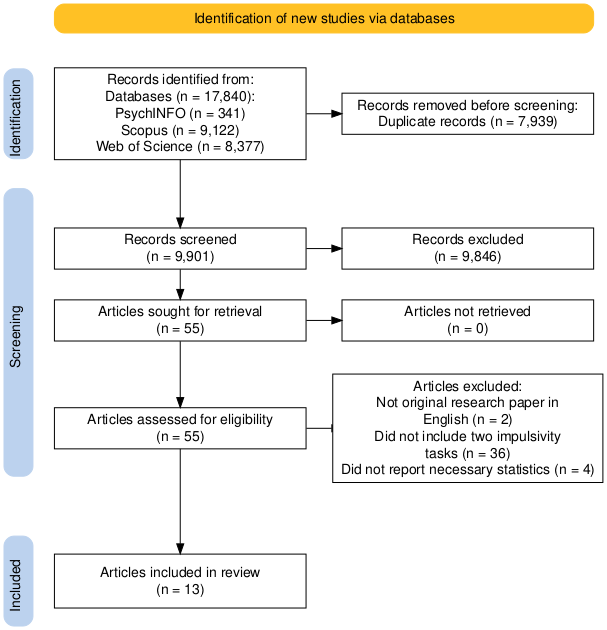
\includegraphics[width=0.8\linewidth]{"figures/prisma_chart.png"}
\end{center}


\end{figure*}

\hypertarget{screening-process-and-exclusion-criteria}{%
\subsection{Screening Process and Exclusion Criteria}\label{screening-process-and-exclusion-criteria}}

To be included in our analysis, reports had to meet several criteria. Only complete, published reports that were available in English in an electronic format were included in the analysis. All reports had to be original, experimental work; observational work was not included. Relevant dissertations were included; however, if duplicate studies existed between dissertations and journal articles, the journal article was included in the analysis.

After our initial database search, we merged results across the three databases and filtered out duplicated records based on DOI or journal information. The remaining 9,901 records were then screened in two phases. First, the title and abstract of each record were screened, and records were excluded if they: (1) did not use domestic dogs as the study subjects, (2) did not use one or more behavioral measures of impulsivity in dogs, or (3) were not experimental research studies. For the purpose of our analysis, we considered a record to use dogs as study subjects when the study incorporated live, behaving domestic dogs. We excluded studies that used only canine tissue/cells or if they investigated only wild canids. If wild canids and domestic dogs were both subjects of a study, the record was included; however, only the data from domestic dogs was analyzed. There were no restrictions on the age, sex, or neuter status of the dogs used in the studies. Records that raised the possibility of inclusion but did not clearly meet the criteria were included for further assessment.

After this first round of screening, we downloaded and evaluated the reports for the remaining 54 records. During this round, reports were excluded if they: (1) were not complete, original reports available in English, (2) did not include either two impulsivity tasks or one impulsivity task and the overall score for the Dog Impulsivity Assessment Scale (DIAS, Wright et al., 2011), or (3) did not report the statistics required to obtain a correlation coefficient. The reports that met the criteria at this point were included in our final group of 13 reports.

\hypertarget{information-extracted-from-studies}{%
\subsection{Information Extracted from Studies}\label{information-extracted-from-studies}}

Our 13 reports comprised 12 journal articles and 1 dissertation. These reports included a total of 17 studies since a record could include multiple studies or study populations (Table \ref{tab:studies}). The final set of studies contained a total of 14 different impulsivity tasks plus the DIAS, which was used in 6 of the studies. Table \ref{tab:tasks} lists the impulsivity tasks included in our analysis, as well as the specific measure used for each task. For each study, we recorded population characteristics when available, including total sample size, numbers of males/females, neuter status of dogs, type of dog (pet, working, free-ranging, captive, or shelter dogs), and whether a specific breed of dog or type of working dog was used as the subject (i.e., border collies, sled working dogs). For each study, we compiled all task pairs---pairwise combinations of tasks and/or task/DIAS combinations---that could result in a correlation coefficient. Some studies had multiple measures for the same task (e.g., accuracy and latency), so we included all measures of all task pairs. This resulted in 63 unique study measures. For each study measure, we recorded the impulsivity task(s) and/or DIAS used in task pair, the type of effect size, the effect size value, the sample size, and whether the authors reported the effect as statistically significant (i.e., \(p\) \textless{} 0.05). To avoid the ``double-counting'' associated with multiple measures for the same task pair (Harrer et al., 2021), we selected a single measure for each task in a pair. To select the measure, we prioritized measures that (1) were used in multiple studies, (2) were scaled in the direction of higher values representing more impulsivity, and (3) were commonly used in the literature. Once we removed extra measures, we had 46 pairs of measures to evaluate.

\renewcommand{\arraystretch}{1.2}

\begin{table*}

\caption{\label{tab:studies}Study Characteristics}
\centering
\fontsize{10}{12}\selectfont
\begin{tabular}[t]{l>{\raggedright\arraybackslash}p{4.75cm}>{\centering\arraybackslash}p{1.1cm}>{\centering\arraybackslash}p{1.1cm}>{\centering\arraybackslash}p{1.1cm}>{\centering\arraybackslash}p{1.25cm}>{\raggedright\arraybackslash}p{4cm}}
\toprule
No. & Study & Sample size & Dog type & Sex ratio & Neutered status & Tasks\\
\midrule
1 & Brady et al. (2018)  Study 1 & 24 & Pet & 14:10 & -- & Spatial Impulsivity, DIAS\\
2 & Brady et al. (2018)  Study 2 & 13 & Pet & 8:5 & -- & Spatial Impulsivity, DIAS\\
3 & Brady et al. (2018)  Study 3 & 23 & Pet & 11:12 & -- & Spatial Impulsivity, DIAS\\
4 & Bray et al. (2014) & 30 & Pet & 15:15 & -- & A-not-B Cup, Cylinder, Social Inhibition\\
5 & Brucks et al. (2017) & 67 & Pet & 34:33 & 40:27 & Box, Buzzer, Delay of Gratification, Middle Cup, DIAS\\
6 & Brucks et al. (2019) & 17 & Captive & 10:7 & -- & Box, Buzzer, Middle Cup\\
7 & Fagnani et al. (2016a) Study 1 & 14 & Pet & 5:9 & -- & A-not-B Cup, Cylinder\\
8 & Fagnani et al. (2016a) Study 2 & 13 & Shelter & 8:5 & -- & A-not-B Cup, Cylinder\\
9 & Fagnani et al. (2016b) & 22 & Pet/ Shelter & 9:13 & -- & Delay Discounting, DIAS\\
10 & Kelly et al. (2019) & 15 & Working & 8:7 & 11:4 & A-not-B Barrier, A-not-B Cup, Cylinder\\
11 & Marshall-Pescini et al. (2015) & 14 & Captive & 7:7 & -- & Cylinder, Detour Fence\\
12 & Mongillo et al. (2019) & 48 & Pet & 24:24 & 24:24 & Spatial Impulsivity, DIAS\\
13 & M\"{u}ller et al. (2016) & 41 & Pet & 6:25 & -- & Leash, Middle Cup, Wait-for-Treat\\
14 & Olsen (2019) Study 1 & 15 & Pet & 9:6 & 15:0 & A-not-B Cup, Cylinder, DIAS\\
15 & Olsen (2019) Study 2 & 34 & Pet & 15:18 & 28:5 & A-not-B Cup, Cylinder, DIAS\\
16 & Vernouillet et al. (2018) & 30 & Pet & 13:17 & -- & A-not-B Barrier, A-not-B Cup, Cylinder, Detour Fence\\
17 & Wright et al. (2012) & 41 & Pet & 17:24 & 30:11 & Delay Discounting, DIAS\\
\bottomrule
\end{tabular}
\end{table*}

\begin{table*}

\caption{\label{tab:tasks}Tasks and Measures}
\centering
\begin{threeparttable}
\begin{tabular}[t]{l>{\raggedright\arraybackslash}p{5.5cm}r}
\toprule
Task & Measure & Study\\
\midrule
A-not-B Barrier & Number of trials before correct & 10, 16\\
A-not-B Cup & First location searched* & 4\\
 & Frequency of errors & \sout{7, 8}\\
 & Number of trials before correct & 7, 8, 10, 14, 15, \vphantom{1} 16\\
Box & Frequency of errors & 5, 6\\
Buzzer & Proximity to box & 5, 6\\
Cylinder & Frequency of errors & \sout{7, 8}\\
 & Number of trials before correct & 7, 8, 10, 14, 15, 16\\
 & Percent correct trials* & 4, 11, \sout{14, 15}\\
Delay Discounting & Maximum delay tolerated* & 9, 17\\
 & Rate of response during delay & \sout{17}\\
Delay of Gratification & Maximum delay tolerated* & 5\\
Detour Fence & Duration of time near fence & \sout{11}\\
 & Latency to reward & 11\\
 & Number of trials before correct & 16\\
Leash & Performance score* & 13\\
Middle Cup & Performance score* & 13\\
 & Ratio correct choices in control/experimental* & 5, 6\\
Sit-Stay & Interval between breaks* & \sout{14}\\
 & Number of breaks & 14\\
 & Time until first break* & \sout{14}\\
Social Inhibition & Difference in choices between control/experimental* & 4\\
Spatial Impulsivity & Maximum distance travelled* & 1, 2, 3\\
 & Percent choosing larger* & 12\\
Wait-for-Treat & Performance score* & 13\\
\bottomrule
\end{tabular}
\begin{tablenotes}
\item \linebreak \textit{Note}. * represents measures scaled with higher values representing less impulsivity. Correlation coefficients for these measures were multiplied by $-$1 to ensure all positive correlations represent higher impulsivity. For studies with multiple measures in a task, \sout{strikethrough} signals removal of the associated measure from the analysis.
\end{tablenotes}
\end{threeparttable}
\end{table*}

\hypertarget{data-reliability}{%
\subsection{Data Reliability}\label{data-reliability}}

After the initial database search, two reviewers (JB and YW) screened the title and abstract of a subset of the records from the first round of screening. First, both reviewers screened 100 randomly chosen records individually. For each record, the reviewers investigated whether the inclusion criteria were met, and, if not, the reason for exclusion was noted. The reviewers then compared their responses, and, after 100\% agreement was reached, the two reviewers split the remaining records for this round of screening. After the first round of screening, the two reviewers screened the remaining 54 papers, focusing on the Methods sections. During this stage, both reviewers individually screened 20 randomly chosen records and decided if each paper met the criteria to be included in the final analysis. If a record did not meet the inclusion criteria, then the reason for exclusion was noted. Once 100\% agreement was reached on whether each paper should be included or the reason for exclusion, a single reviewer (JB) screened the remaining records. This reviewer also extracted and recorded the required data from each record.

\hypertarget{transparency-and-openness}{%
\subsection{Transparency and Openness}\label{transparency-and-openness}}

We report how we determined our sample size, all data exclusions (if any), all manipulations, and all measures in the study. We analyzed data from the project using R (Version 4.2.2; R Core Team, 2022) and the R-packages \emph{here} (Version 1.0.1; Müller, 2020), \emph{kableExtra} (Version 1.3.4; Zhu, 2021), \emph{knitr} (Version 1.41; Xie, 2015), \emph{lubridate} (Version 1.9.0; Grolemund \& Wickham, 2011), \emph{papaja} (Version 0.1.1; Aust \& Barth, 2022), \emph{PRISMA2020} (Version 1.0.1; Haddaway et al., 2022), \emph{readxl} (Version 1.4.1; Wickham \& Bryan, 2022), \emph{RoBMA} (Version 2.3.1; Bartoš \& Maier, 2020), \emph{robvis} (Version 0.3.0.900; McGuinness \& Higgins, 2020), and \emph{tidyverse} (Version 1.3.2; Wickham et al., 2019). The manuscript was created using \emph{rmarkdown} (Version 2.19, Xie et al., 2018) and \emph{papaja} (Version 0.1.1, Aust \& Barth, 2022). Data, analysis scripts, supplementary materials, and reproducible research materials are available at the Open Science Framework (\url{https://osf.io/z6svt/}). We pre-registered our design and analysis plan at the Open Science Framework (\url{https://osf.io/bsyxk}).

\hypertarget{data-analysis}{%
\subsection{Data Analysis}\label{data-analysis}}

The first step in our data analysis was to convert any other types of effect sizes to correlation coefficients. All effect sizes were already presented as correlation coefficients, though some were presented as Pearson correlations and other Spearman correlations. For measures scaled such that higher values meant \emph{less} impulsivity, we reversed the sign of the correlation coefficient (if both measures in a correlation were scaled this way, we reversed the sign twice). Thus, all correlation coefficients represented \emph{more} impulsivity for both tasks.

Our first analysis generated a matrix of the effect sizes for all impulsivity task pairs. Within each cell of (half of) the matrix, we aggregate the correlation coefficient, sample size, and citation for each study that correlates that pair of tasks.

For any cell in the table that had three or more studies in it, we conducted a robust Bayesian, model-averaged meta-analysis. We input the correlation coefficients and sample sizes into the \texttt{RoBMA()} function in the \emph{RoBMA} package (Bartoš \& Maier, 2020), using default priors (standard normal distribution on effect sizes, inverse gamma distribution with \(\alpha\) = 1 and \(\beta\) = 0.15 on heterogeneity, two two-sided weight functions with cut-points at (0.05) and (0.05, 0.10) and parameters \(\alpha\) = (1, 1) and (1, 1, 1), and the default point priors on the null hypotheses) (Bartoš et al., 2022). This function allows us to test not only if there is evidence of an effect but also evidence for between-study heterogeneity (whether there is variation in true effect sizes across studies) and publication bias (Maier et al., 2022). This analysis used model averaging to calculate (1) a Bayesian estimate of the effect size across all studies, (2) a Bayes factor for evidence supporting the hypothesis of an effect, (3) a Bayes factor for evidence supporting the presence of between-study heterogeneity, and (4) a Bayes factor for evidence supporting the presence of publication bias (Maier et al., 2022). We set the prior hypothesis probability to 0.50 for the effect size, heterogeneity, and publication bias.

\hypertarget{results}{%
\section{Results}\label{results}}

Our first analysis aggregated all of the correlation coefficients for each pair of tasks or task/DIAS pair for each study (Table \ref{tab:taskpairs}). Across 46 task/task or task/DIAS pairs, study authors reported 38 pairs as not demonstrating a statistically significant correlation and 8 pairs as demonstrating a correlation. For only the 31 task/task pairs, 28 were not correlated, while 3 were correlated. For only the 15 task/DIAS pairs, 10 were not correlated, while 5 were correlated. Thus, the vast majority of task/task pairs show no correlations. Notably, one of the three task/task correlations was between two versions of the same task: A-not-B Barrier and A-not-B Cup. Also, the other two task correlations included the Wait-for-Treat task. The task/DIAS correlation fared better with DIAS overall scores correlating with A-not-B Cup, Delay Discounting, Delay of Gratification, and Spatial Impulsivity.

\begin{landscape}\begin{table}

\caption{\label{tab:taskpairs}Task Pair Correlations}
\centering
\resizebox{\linewidth}{!}{
\fontsize{8}{10}\selectfont
\begin{threeparttable}
\begin{tabular}[t]{>{\raggedright\arraybackslash}p{1.6cm}>{\raggedright\arraybackslash}p{2.3cm}>{\raggedright\arraybackslash}p{1.8cm}>{\raggedright\arraybackslash}p{2.2cm}>{\raggedright\arraybackslash}p{1.9cm}>{\raggedright\arraybackslash}p{2.2cm}>{\raggedright\arraybackslash}p{2cm}>{\raggedright\arraybackslash}p{2.1cm}>{\raggedright\arraybackslash}p{1.9cm}>{\raggedright\arraybackslash}p{2.2cm}>{\raggedright\arraybackslash}p{2.3cm}}
\toprule
Task & A-not-B Cup & Buzzer & Cylinder & Delay of Gratification & Detour Fence & Middle Cup & Sit-Stay & Social Inhibition & Wait-for-Treat & DIAS\\
\midrule
A-not-B Barrier & \textbf{$\rho_{(15)}$=0.60 [10]*},\newline $\rho_{(30)}$=0.18 [16] &  & $\rho_{(15)}$=$-$0.10 [10],\newline $\rho_{(30)}$=0.21 [16] &  & $\rho_{(30)}$=0.11 [16] &  &  &  &  & \\
\addlinespace
A-not-B Cup &  &  & $\rho_{(30)}$=0.11 [4],\newline $\rho_{(14)}$=$-$0.13 [7],\newline $\rho_{(13)}$=$-$0.04 [8],\newline $\rho_{(15)}$=$-$0.45 [10],\newline $\rho_{(15)}$=0.01 [14],\newline $\rho_{(34)}$=$-$0.08 [15],\newline $\rho_{(30)}$=$-$0.15 [16] &  & $\rho_{(30)}$=$-$0.06 [16] &  & $\rho_{(15)}$=0.28 [14] & $\rho_{(30)}$=0.04 [4] &  & \textbf{$\rho_{(15)}$=0.61 [14]*},\newline $r_{(34)}$=0.40 [15]\\
\addlinespace
Box &  & $\rho_{(67)}$=0.14 [5],\newline $\rho_{(17)}$=0.37 [6] &  & $\rho_{(67)}$=$-$0.15 [5] &  & $\rho_{(67)}$=$-$0.02 [5],\newline $\rho_{(17)}$=0.17 [6] &  &  &  & $\rho_{(67)}$=0.15 [5]\\
\addlinespace
Buzzer &  &  &  & $\rho_{(67)}$=$-$0.28 [5] &  & $\rho_{(67)}$=0.12 [5],\newline $\rho_{(17)}$=0.08 [6] &  &  &  & $\rho_{(67)}$=$-$0.10 [5]\\
\addlinespace
Cylinder &  &  &  &  & $\rho_{(14)}$=$-$0.13 [11],\newline $\rho_{(30)}$=$-$0.09 [16] &  & $\rho_{(15)}$=$-$0.50 [14] & $\rho_{(30)}$=$-$0.06 [4] &  & $\rho_{(15)}$=$-$0.21 [14],\newline $\rho_{(34)}$=0.05 [15]\\
\addlinespace
Delay Discounting &  &  &  &  &  &  &  &  &  & $\rho_{(22)}$=$-$0.12 [9],\newline \textbf{$r_{(41)}$=0.65 [17]*}\\
\addlinespace
Delay of Gratification &  &  &  &  &  & $\rho_{(67)}$=0.07 [5] &  &  &  & \textbf{$\rho_{(67)}$=0.39 [5]*}\\
\addlinespace
Leash &  &  &  &  &  & $\rho_{(41)}$=0.23 [13] &  &  & \textbf{$\rho_{(41)}$=0.45 [13]*} & \\
\addlinespace
Middle Cup &  &  &  &  &  &  &  &  & \textbf{$\rho_{(41)}$=0.33 [13]*} & $\rho_{(67)}$=0.01 [5]\\
\addlinespace
Sit-Stay &  &  &  &  &  &  &  &  &  & $\rho_{(15)}$=0.48 [14]\\
\addlinespace
Spatial Impulsivity &  &  &  &  &  &  &  &  &  & \textbf{$r_{(24)}$=0.46 [1]*},\newline \textbf{$r_{(13)}$=0.61 [2]*},\newline $r_{(23)}$=0.05 [3],\newline $r_{(48)}$=$-$0.01 [12]\\
\bottomrule
\end{tabular}
\begin{tablenotes}
\small
\item \linebreak \textit{Note}. Cells include correlation coefficient type (Pearson's $r$ or Spearman's $\rho$), sample size (in parenthesis), correlation coefficient value, and study number [in brackets]. Correlation coefficients reported with $p < 0.05$ are \textbf{bolded with an asterisk*}. Correlation coefficients were multiplied by $-$1 to ensure all positive correlations represent higher impulsivity for both tasks. DIAS is the Dog Impulsivity Assessment Scale (Wright et al., 2011).
\end{tablenotes}
\end{threeparttable}}
\end{table}
\end{landscape}

Only two task pairs included three or more studies, thereby meeting our criterion for conducting a formal meta-analysis. Because one of those pairs (Spatial Impulsivity and DIAS) has recently had a meta-analysis conducted, with new studies published after our search deadline (Stevens et al., 2022), we did not conduct a meta-analysis for that pair. To summarize Stevens et al. (2022), two out of six studies found a correlation between Spatial Impulsivity and DIAS scores. A Bayesian, model-averaged meta-analysis found anecdotal evidence of no correlation between Spatial Impulsivity and DIAS scores, but further studies are needed to confirm this result.

The other task pair with more than two studies was A-not-B Cup and Cylinder. None of the seven studies that tested both of these tasks on the same dog reported a statistically significant correlation. Robust Bayesian meta-analysis found moderate evidence against the effect, \(BF_{10}\) = 0.270, with mean model-averaged estimate correlation = -0.017, 95\% CI {[}-0.200, 0.034{]}. Robust Bayesian meta-analysis found weak evidence against the heterogeneity, \(BF_{10}\) = 0.563, with mean model-averaged estimate tau = 0.028, 95\% CI {[}0.000, 0.171{]} and moderate evidence against publication bias, \(BF_{10}\) = 0.284. Thus, there was no evidence for a correlation in responses between the A-not-B Cup and Cylinder tasks (Figure \ref{fig:forest}). Further, there was no evidence for publication bias favoring studies that found a correlation. Even when correcting for publication bias, the conditional PET-PEESE estimate of the overall effect does not differ from 0 (\textbf{PET}-PEESE: 0.013 {[}0.000, 0.140{]}). And there was weak evidence against between-study heterogeneity, suggesting that the effect sizes are relatively homogeneous across studies, despite using different measures within the tasks.

\begin{figure*}
\caption{\newline Meta-Analysis Forest Plot for A-not-B Cup and Cylinder Tasks \label{fig:forest}}
\begin{center}
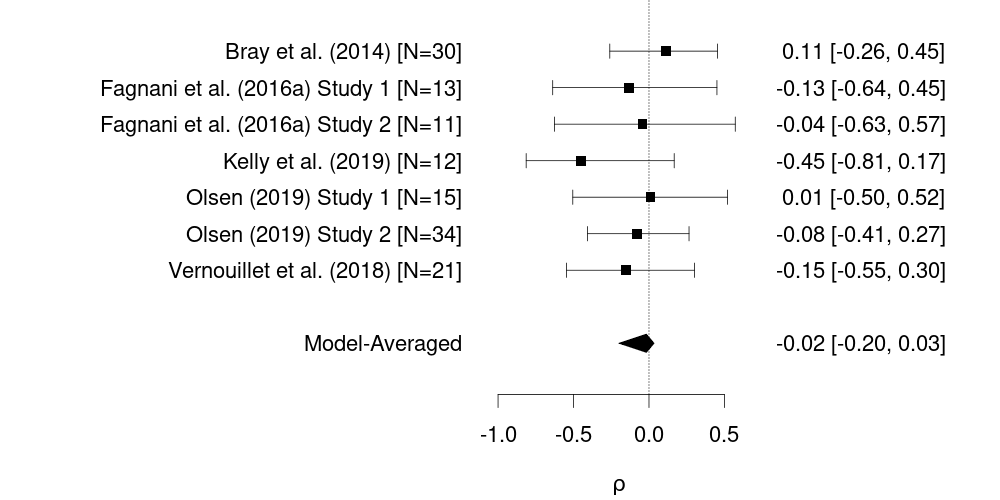
\includegraphics[width=0.8\linewidth]{"figures/anotb-cylinder-forestplot.png"}
\end{center}


\end{figure*}

\hypertarget{discussion}{%
\section{Discussion}\label{discussion}}

We examined almost 10,000 bibliographic records to discover 13 reports that tested multiple impulsivity tasks or owner surveys of dog impulsivity within the same dogs. This resulted in 46 task/task or task/survey pairs of which only 8 found a correlation. Correlations were more common between tasks and the survey than between different tasks. We also conducted a formal meta-analysis for correlations between the A-not-B Cup task and Cylinder task (N=7 studies). We found no evidence for a correlation in performance between these two tasks. Thus, overall, our systematic review and meta-analysis found little evidence for consistent relationships between impulsivity levels across tasks.

\hypertarget{implications}{%
\subsection{Implications}\label{implications}}

For the 31 task/task pairs (not including DIAS survey data), only 3 (9.7\%) were correlated. One of the correlated pairs involved the A-not-B Barrier and A-not-B Cup task (Kelly et al., 2019). It is therefore not surprising that two similar tasks result in consistent performance. Moreover, this study only tested 15 dogs, and small sample sizes can result in inflated effect sizes (Gelman \& Carlin, 2014). A separate study comparing these two tasks with a larger sample size did not find a correlation (Vernouillet et al., 2018). The other two correlated pairs both involved the Wait-for-Treat task (Müller et al., 2016). In this task, a treat was placed in front of the dog, a ``wait'' command was given, and the dog was supposed to wait for a ``go'' command before retrieving the treat. Though this task clearly requires inhibition, performance may reflect training more than impulsivity (Müller et al., 2016). Thus, even in the cases where we observe correlations between impulsivity tasks, they occur for small sample sizes, with similar tasks, and when training may account for performance.

The lack of correlations across tasks may seem surprising. However, work in human impulsivity also shows that different impulsivity tasks and surveys do not combine into a single behavioral trait (Malle \& Neubauer, 1991; Wingrove \& Bond, 1997; Smith et al., 2007). MacKillop et al. (2016) separated out impulsive action (the failure to inhibit an action or the ability to withhold from making a response) from impulsive choice (choosing between rewards with different costs) and impulsive personality traits (self-reported attributions of self-regulatory capacity). Though the authors found correlations between tasks within the categories, they did not find correlations between categories. A review of the construct of impulsivity in human studies corroborates distinct subtypes of impulsivity (Dick et al., 2010). However, a key difference between human and animal work is that, while humans do show correlations between tasks \emph{within} the subtypes of impulsivity (e.g., impulsive action and impulsive choice), animal works shows that different tasks within a subtype are not necessarily related in rats (Peterson et al., 2015) or primates (Addessi et al., 2013). Indeed, our meta-analysis of performance in A-not-B Cup and Cylinder tasks (tasks within the impulsive action subtype) showed no correlation across seven studies (Figure \ref{fig:forest}). Even the similar Cylinder and Detour Fence tasks---which both involve motor inhibition of not moving directly toward food but instead detouring around a transparent obstacle---are not correlated in two studies. In fact, the Cylinder task was used in 13 different studies (12 of which were impulsive action tasks) but did not correlate with any of them. Thus, even within a subtype of impulsivity, animals do not show strong evidence for the behavioral trait of impulsivity, and dogs seem to follow this pattern.

Though behavioral tasks do not seem to correlate, it is possible for dog owners to extract a `personality trait' from their dog's behavior. The DIAS provides a survey for owners to do just that. For the 15 task/DIAS survey pairs, owner reports of impulsivity were correlated in 5 (33.3\%) studies over four different tasks: A-not-B Cup, Delay Discounting, Delay of Gratification, and Spatial Impulsivity. This is obviously a higher rate than that observed between behavioral tasks. Three of these studies with correlations were conducted by the authors of the DIAS (Wright et al., 2012; Brady et al., 2018), but two studies were independent of the DIAS authors (Brucks et al., 2017; Olsen, 2019). Two of these studies (A-not-B Cup and Spatial Impulsivity) used small sample sizes (N=13--15), raising the possibility of inflated effect sizes. For both tasks, studies with larger sample sizes failed to find correlations (A-not-B Cup, Olsen, 2019; Spatial Impulsivity: Mongillo et al., 2019). Further replications of the Spatial Impulsivity studies not included here (due to publication after the search deadline) also failed to find a correlation between owner perceived impulsivity and performance on the Spatial Impulsivity tasks (Stevens et al., 2022). Moreover, a Bayesian meta-analysis of all six studies found anecdotal evidence of no correlation between DIAS and Spatial Impulsivity performance. Interestingly, DIAS scores correlated with performance in the Delay Discounting (Wright et al., 2012) and Delay of Gratification (Brucks et al., 2017) tasks, two classic tasks for assessing intertemporal choice, or preferences for immediate vs.~delayed rewards.

For task/DIAS pairs, 4 of the 5 correlations occurred for tasks associated with impulsive choice: Delay Discounting, Delay of Gratification, and Spatial Impulsivity. In this case, smaller, sooner or closer rewards vs.~larger, later or more distant rewards. This is perhaps surprising given that only 1 of the 18 DIAS questions references aspects of intertemporal or spatial choice (``Dog is not very patient''). In fact, most of the DIAS questions do not directly ask about impulsivity unless they do so in a general way (``Dog is considered to be very impulsive'') or by focusing on impulsive action (``Dog does not think before it acts'', ``Dog appears to have a lot of control over how it responds''). Most DIAS questions reference excitement, persistence, trainability, aggression, neophobia, and reactivity. Therefore, it remains unclear what aspects of dog behavior the DIAS is capturing in its assessment of impulsivity.

In summary, we do not have strong evidence for impulsivity as a single behavioral trait. Perhaps this is not surprising given the multifaceted nature of impulsivity and the few correlations that we observe between tasks in humans and other species. Yet characterizing impulsivity as a behavioral trait---if it exists---could be useful for canine science, as often dog owners and handlers want dogs to inhibit their impulses. And we have some evidence of impulsivity mapping onto important behavior in working dogs. Impulsivity (measured via inhibition in the Cylinder task) was associated with success in an explosive detection task in a population of police explosive search dogs (Tiira et al., 2020). Persistence and problem solving were not associated with their detection success. Lazarowski et al. (2020) did not find a relationship between Cylinder task success and detection dog performance, but they did find that success in an A-not-B Barrier task was associated with performance. Thus, the ability to inhibit impulsivity in behavioral tasks may predict real-world performance for working dogs. This relationship suggests that assessing impulsivity may help in the selection of working dogs for training programs.

\hypertarget{limitations}{%
\subsection{Limitations}\label{limitations}}

While systematic reviews and meta-analyses can be a useful way to aggregate the literature to examine larger-scale patterns, they also come with limitations. Of course, one of the primary and most nefarious limitations is publication bias---only a subset of studies end up getting published, and often the published studies are biased toward demonstrating effects (Scherer et al., 2018; Siddaway et al., 2019; Harrer et al., 2021). Interestingly, for this review, only 17.4\% of the tested task pairs or task/survey pairs reported statistically significant effects. So though publication bias is possible, it might not be as pervasive as it is in other areas. Furthermore, a direct test for publication bias in the A-not-B Cup and Cylinder task comparisons showed no evidence for publication bias.

A larger problem for this review is the quality of the data in the literature. Individual studies can vary in sample sizes, methodological rigor, and generalizability, which can lead to biasing the outcomes of systematic reviews and meta-analysis (Siddaway et al., 2019; Harrer et al., 2021). Therefore, researchers have developed \emph{risk of bias} criteria to score individual studies. Here, we used Nudelman and Otto's (2020) generic Risk of Bias Utilized for Surveys Tool (ROBUST) to assess the studies included in our review. This tool categorizes the risk of bias for the following criteria: sampling frame (correspondence between theoretical population and sampled population), participant recruitment (description of subject recruitment), acceptability of exclusion rate, sufficiency of sample size, demographic variables (reporting of demographic information), reliability of measurements, setting (appropriateness of experimental setting), and data management (appropriate dealing with outliers, missing data) (see in-depth description of each criterion in Supplementary Materials). We categorized each study for each criterion (Figure S1). In general, the studies had relatively low risk of bias for most criteria (Figure S2). By far the greatest risk of bias resulted from low sample sizes---most of the studies analyzed here had fewer than 25 subjects (Table \ref{tab:studies}; Figure S3). Correlations are notoriously unstable with small sample sizes, resulting in multiple types of inferential errors (Schönbrodt \& Perugini, 2013; Gelman \& Carlin, 2014; Knudson \& Lindsey, 2014). Therefore, it is possible both that statistically significant correlations are false positives and that statistically non-significant correlations are false negatives. In our data, for three tasks pairs with multiple studies and significant correlations, the study with the larger sample size was non-significant (Table \ref{tab:taskpairs}). In one task pair, the larger sample size study showed a correlation, while the smaller did not. Of course, other factors could contribute to these differences, but a key aim of canine behavioral science should be to increase sample sizes to improve robustness of results.

Another key potential contributor to bias is the reliability of the measures. One surprising outcome from this review was the variation in different measures used for the same task. Four of the tasks had three different measures for the same task, sometimes between studies, sometimes within studies (Table \ref{tab:tasks}). For our aggregation and meta-analysis, we selected a single measure for each task pair. We prioritized measures that were used in multiple studies, were scaled in the direction of higher values representing more impulsivity, and were commonly used in the literature. While not an arbitrary choice, these selection rules could have biased our results, and other measures might have resulted in different outcomes. In addition to measure selection, measure quality is important as well. Measures vary in their precision, variability, and objectivity. For example, for the A-not-B Cup task, the measure of \emph{first location search} is limited in its variability because there are only two or three possible outcomes, limiting the variability needed for robust correlations. The measure of \emph{number of trials before correct}, however, is a count of trial numbers (0 to infinity), so it has the potential for more variability. Lastly, measures include uncertainty, and single point estimates may not accurately capture the underlying construct. Almost all of the studies included here (with the exception of Brady et al., 2018) did not include test-retest validation of their measures. Therefore, the measure values may lack precision, making the correlations less accurate.

Only two task pairs included enough studies to warrant meta-analysis. One of those pairs has recently had a meta-analysis (Stevens et al., 2022), so we only conducted a single meta-analysis here: A-not-B Cup and Cylinder. A key limitation of this analysis is the number of studies included---only seven. Though this is relatively high for repeated studies in canine behavioral science, meta-analytic methods, especially estimating between-study heterogeneity, perform better with more studies included (Harrer et al., 2021). Other studies (Lazarowski et al., 2020; Tiira et al., 2020) have tested both A-not-B Cup and Cylinder in the same dogs, but they did not report the effect size (though both sets of authors state there was no correlation). Similarly, other studies measured A-not-B Cup/DIAS (Cavalli et al., 2018) and Spatial Impulsivity/DIAS (Riemer et al., 2014) without reporting correlation coefficients. We recommend authors always report effect sizes for these correlations with an eye toward future meta-analyses.

\hypertarget{future-directions}{%
\subsection{Future directions}\label{future-directions}}

Impulsivity is closely tied to aspects of canine-human interaction: from detection dogs inhibiting the impulse to track non-target scents to pet dogs avoiding eating the scrumptious food (to them) but disgusting waste (to us) while on walks. Much of dog training focuses on impulse control. Thus, the line between impulsivity as a personality trait and a trained behavior is blurred. This, therefore, could result in variation from dogs being differently trained for impulse control, where the training generalizes more to some impulsivity tasks than others. The close relationship between impulsivity and training has two important implications going forward. First, we need to think more carefully about the construct of impulsivity, its different subtypes, and its susceptibility to training. Is the impulsive action/choice distinction sufficient for categorizing impulsivity, or do we need a more nuanced approach? When training impulse control, does this apply uniformly across all subtypes of impulsivity, or does it focus in on particular subtypes, thereby breaking any potential relationship across tasks? Second, given the strong connection between training and impulsivity, we must be more sophisticated in collecting data on training for individual dogs. The current general surveys on training (e.g., C-BARQ, Hsu \& Serpell, 2003) may not be nuanced enough to properly measure impulse control training. We need to focus more effort on understanding the relationships between impulsivity and training.

In a previous meta-analysis of correlations between spatial impulsivity performance and owner perception of impulsivity (via the DIAS survey), different research labs produced different outcomes (Stevens et al., 2022). One of the more interesting possible explanations for these mixed results is potential cultural differences between study populations. Those studies occurred in the United Kingdom, Italy, and the United States. Residents of different countries have different attitudes about, interactions with, and experience with training their dogs (Bradshaw \& Goodwin, 1999; Serpell, 2004; Wan et al., 2009; Amici et al., 2019). A key cultural difference relevant here is the frequency of spaying/neutering (Diesel et al., 2010; Trevejo et al., 2011), because neutering may influence impulsivity (Fadel et al., 2016). Thus, cultural differences should be accounted for when studying canine behavioral science. One solution to this is to engage in big team science. The ManyDogs Project is a consortium of dog behavior researchers interested in conducting the same study across many labs all over the world (ManyDogs Project et al., 2022). Since different breeds may show different levels of impulsivity (Junttila et al., 2022), large sample sizes may address sampling variability problems cause by differences in breed compositions across studies. Implementing impulsivity tasks and the DIAS across a wide range of labs will not only overcome the low sample size problem rampant in this area but also allows the analysis of potential cultural differences.

An active area of research in human and rat impulsivity explores the mechanisms underlying this construct (Robbins \& Dalley, 2017). Though studies of genetic (Hejjas et al., 2007; Kubinyi et al., 2012), neural (Cook et al., 2016), and hormonal (Rayment et al., 2020; Junttila et al., 2021) mechanisms of impulsivity are increasing in canine science, we lack a coherent research program on the underpinnings of impulsivity in dogs, and further investigations in this area could be a fruitful area of research (Olsen, 2018). Understanding the genetic, neural, and hormonal influences on impulsivity has critical implications for the breeding, selection, and training of not only pet dogs but also working and service dogs.

\hypertarget{conclusion}{%
\subsection{Conclusion}\label{conclusion}}

Currently, we have little evidence for a behavioral trait of impulsivity in dogs. Performance rarely correlates across impulsivity tasks, and owner perceptions of impulsivity often do not match behavioral measures. This may not be too surprising given what we know about the multifaceted nature of impulsivity and the lack of strong signals of a trait in humans and other animals. Moreover, dog owners and handlers expressly train for impulse control, potentially interfering with our ability to accurately measure it as a trait. Further, many of the studies evaluating impulsivity in dogs suffer from small sample sizes, which can lead to weak statistical analyses. Larger-scale studies with a clearer conceptual foundation for the nature of impulsivity and robust measures of impulsivity are needed to verify whether impulsive action and choice do carry over across contexts. Understanding the extent and limits of impulsivity in dogs is critical to the canine-human bond.

\hypertarget{author-contributions}{%
\subsection{Author Contributions}\label{author-contributions}}

JB: Data curation, Investigation, Methodology, Project administration, Validation, Writing -- original draft; YW: Investigation, Validation; JS: Conceptualization, Data curation, Formal analysis, Funding acquisition, Methodology, Project administration, Resources, Software, Supervision, Visualization, Writing -- original draft.

\hypertarget{conflict-of-interest}{%
\subsection{Conflict of interest}\label{conflict-of-interest}}

The authors declared that no conflicts of interest exist.

\hypertarget{data-availability}{%
\subsection{Data Availability}\label{data-availability}}

The data and analysis code are available at: \url{https://osf.io/z6svt/}.

\hypertarget{ethics-statement}{%
\subsection{Ethics statement}\label{ethics-statement}}

An ethics statement is not applicable because this study is based exclusively on published literature.

\hypertarget{references}{%
\section{References}\label{references}}

\scriptsize

\hypertarget{refs}{}
\begin{CSLReferences}{1}{0}
\leavevmode\vadjust pre{\hypertarget{ref-Addessi.etal.2013}{}}%
Addessi, E., Paglieri, F., Beran, M. J., Evans, T. A., Macchitella, L., De Petrillo, F., \& Focaroli, V. (2013). Delay choice versus delay maintenance: Different measures of delayed gratification in capuchin monkeys (\emph{{Cebus} apella}). \emph{Journal of Comparative Psychology}, \emph{127}(4), 392--398. \url{https://doi.org/10.1037/a0031869}

\leavevmode\vadjust pre{\hypertarget{ref-Amici.etal.2019}{}}%
Amici, F., Waterman, J., Kellermann, C. M., Karimullah, K., \& Bräuer, J. (2019). The ability to recognize dog emotions depends on the cultural milieu in which we grow up. \emph{Scientific Reports}, \emph{9}(1), 1--9. \url{https://doi.org/10.1038/s41598-019-52938-4}

\leavevmode\vadjust pre{\hypertarget{ref-R-papaja}{}}%
Aust, F., \& Barth, M. (2022). \emph{{papaja}: {Prepare} reproducible {APA} journal articles with {R Markdown}}. \url{https://github.com/crsh/papaja}

\leavevmode\vadjust pre{\hypertarget{ref-Barela.etal.2023}{}}%
Barela, J., Worth, Y., \& Stevens, J. R. (2023). \emph{Impulsivity as a trait in domestic dogs ({Canis} familiaris): A systematic review and meta-analysis}. PsyArXiv. \url{https://doi.org/10.31234/osf.io/ctfns}

\leavevmode\vadjust pre{\hypertarget{ref-R-RoBMA}{}}%
Bartoš, F., \& Maier, M. (2020). \emph{RoBMA: An {R} package for robust {Bayesian} meta-analyses}. \url{https://CRAN.R-project.org/package=RoBMA}

\leavevmode\vadjust pre{\hypertarget{ref-Bartos.etal.2022}{}}%
Bartoš, F., Maier, M., Quintana, D. S., \& Wagenmakers, E.-J. (2022). Adjusting for publication bias in {JASP} and {R}: Selection models, {PET-PEESE}, and robust {Bayesian} meta-analysis. \emph{Advances in Methods and Practices in Psychological Science}, \emph{5}(3), 25152459221109259. \url{https://doi.org/10.1177/25152459221109259}

\leavevmode\vadjust pre{\hypertarget{ref-Batt.etal.2008}{}}%
Batt, L. S., Batt, M. S., Baguley, J. A., \& McGreevy, P. D. (2008). Factors associated with success in guide dog training. \emph{Journal of Veterinary Behavior}, \emph{3}(4), 143--151. \url{https://doi.org/10.1016/j.jveb.2008.04.003}

\leavevmode\vadjust pre{\hypertarget{ref-Bensky.etal.2013}{}}%
Bensky, M. K., Gosling, S. D., \& Sinn, D. L. (2013). The world from a dog's point of view: A review and synthesis of dog cognition research. In H. J. Brockmann, T. J. Roper, M. Naguib, J. C. Mitani, L. W. Simmons, \& L. Barrett (Eds.), \emph{Advances in the {Study} of {Behavior}} (Vol. 45, pp. 209--406). {Academic Press}. \url{https://doi.org/10.1016/B978-0-12-407186-5.00005-7}

\leavevmode\vadjust pre{\hypertarget{ref-Bradshaw.Goodwin.1999}{}}%
Bradshaw, J. W. S., \& Goodwin, D. (1999). Determination of behavioural traits of pure-bred dogs using factor analysis and cluster analysis; a comparison of studies in the {USA} and {UK}. \emph{Research in Veterinary Science}, \emph{66}(1), 73--76. \url{https://doi.org/10.1053/rvsc.1998.0246}

\leavevmode\vadjust pre{\hypertarget{ref-Brady.etal.2018}{}}%
Brady, K., Hewison, L., Wright, H., Zulch, H., Cracknell, N., \& Mills, D. (2018). A spatial discounting test to assess impulsivity in dogs. \emph{Applied Animal Behaviour Science}, \emph{202}, 77--84. \url{https://doi.org/10.1016/j.applanim.2018.01.003}

\leavevmode\vadjust pre{\hypertarget{ref-Bray.etal.2014}{}}%
Bray, E. E., MacLean, E. L., \& Hare, B. A. (2014). Context specificity of inhibitory control in dogs. \emph{Animal Cognition}, \emph{17}(1), 15--31. \url{https://doi.org/10.1007/s10071-013-0633-z}

\leavevmode\vadjust pre{\hypertarget{ref-Brucks.etal.2019}{}}%
Brucks, D., Marshall-Pescini, S., \& Range, F. (2019). Dogs and wolves do not differ in their inhibitory control abilities in a non-social test battery. \emph{Animal Cognition}, \emph{22}(1), 1--15. \url{https://doi.org/10.1007/s10071-018-1216-9}

\leavevmode\vadjust pre{\hypertarget{ref-Brucks.etal.2017a}{}}%
Brucks, D., Marshall-Pescini, S., Wallis, L. J., Huber, L., \& Range, F. (2017). Measures of dogs' inhibitory control abilities do not correlate across tasks. \emph{Frontiers in Psychology}, \emph{8}, 849. \url{https://doi.org/10.3389/fpsyg.2017.00849}

\leavevmode\vadjust pre{\hypertarget{ref-Cavalli.etal.2018}{}}%
Cavalli, C. M., Carballo, F., Dzik, M. V., Underwood, S., \& Bentosela, M. (2018). Are animal-assisted activity dogs different from pet dogs? {A} comparison of their sociocognitive abilities. \emph{Journal of Veterinary Behavior}, \emph{23}, 76--81. \url{https://doi.org/10.1016/j.jveb.2017.12.001}

\leavevmode\vadjust pre{\hypertarget{ref-Cook.etal.2016a}{}}%
Cook, P. F., Spivak, M., \& Berns, G. (2016). Neurobehavioral evidence for individual differences in canine cognitive control: An awake {fMRI} study. \emph{Animal Cognition}, \emph{19}(5), 867--878. \url{https://doi.org/10.1007/s10071-016-0983-4}

\leavevmode\vadjust pre{\hypertarget{ref-Dick.etal.2010}{}}%
Dick, D. M., Smith, G., Olausson, P., Mitchell, S. H., Leeman, R. F., O'Malley, S. S., \& Sher, K. (2010). Understanding the construct of impulsivity and its relationship to alcohol use disorders. \emph{Addiction Biology}, \emph{15}(2), 217--226. \url{https://doi.org/10.1111/j.1369-1600.2009.00190.x}

\leavevmode\vadjust pre{\hypertarget{ref-Diesel.etal.2010}{}}%
Diesel, G., Brodbelt, D., \& Laurence, C. (2010). Survey of veterinary practice policies and opinions on neutering dogs. \emph{Veterinary Record}, \emph{166}(15), 455--458. \url{https://doi.org/10.1136/vr.b4798}

\leavevmode\vadjust pre{\hypertarget{ref-Evenden.1999a}{}}%
Evenden, J. L. (1999). Varieties of impulsivity. \emph{Psychopharmacology}, \emph{146}(4), 348--361. \url{https://doi.org/10.1007/PL00005481}

\leavevmode\vadjust pre{\hypertarget{ref-Fadel.etal.2016}{}}%
Fadel, F. R., Driscoll, P., Pilot, M., Wright, H., Zulch, H., \& Mills, D. (2016). Differences in trait impulsivity indicate diversification of dog breeds into working and show lines. \emph{Scientific Reports}, \emph{6}(1), 22162. \url{https://doi.org/10.1038/srep22162}

\leavevmode\vadjust pre{\hypertarget{ref-Fagnani.etal.2016a}{}}%
Fagnani, J., Barrera, G., Carballo, F., \& Bentosela, M. (2016a). Is previous experience important for inhibitory control? {A} comparison between shelter and pet dogs in {A-not-B} and cylinder tasks. \emph{Animal Cognition}, \emph{19}(6), 1165--1172. \url{https://doi.org/10.1007/s10071-016-1024-z}

\leavevmode\vadjust pre{\hypertarget{ref-Fagnani.etal.2016}{}}%
Fagnani, J., Barrera, G., Carballo, F., \& Bentosela, M. (2016b). Tolerance to delayed reward tasks in social and non-social contexts. \emph{Behavioural Processes}, \emph{130}, 19--30. \url{https://doi.org/10.1016/j.beproc.2016.06.011}

\leavevmode\vadjust pre{\hypertarget{ref-Fratkin.etal.2013}{}}%
Fratkin, J. L., Sinn, D. L., Patall, E. A., \& Gosling, S. D. (2013). Personality consistency in dogs: {A} meta-analysis. \emph{PLOS ONE}, \emph{8}(1), e54907. \url{https://doi.org/10.1371/journal.pone.0054907}

\leavevmode\vadjust pre{\hypertarget{ref-Gelman.Carlin.2014}{}}%
Gelman, A., \& Carlin, J. (2014). Beyond power calculations: {Assessing} type {S} (sign) and type {M} (magnitude) errors. \emph{Perspectives on Psychological Science}, \emph{9}(6), 641--651. \url{https://doi.org/10.1177/1745691614551642}

\leavevmode\vadjust pre{\hypertarget{ref-R-lubridate}{}}%
Grolemund, G., \& Wickham, H. (2011). Dates and times made easy with {lubridate}. \emph{Journal of Statistical Software}, \emph{40}(3), 1--25. \url{https://www.jstatsoft.org/v40/i03/}

\leavevmode\vadjust pre{\hypertarget{ref-R-PRISMA2020}{}}%
Haddaway, N. R., Page, M. J., Pritchard, C. C., \& McGuinness, L. A. (2022). PRISMA2020: An {R} package and {Shiny} app for producing PRISMA 2020-compliant flow diagrams, with interactivity for optimised digital transparency and open synthesis. \emph{Campbell Systematic Reviews}, \emph{18}(2), e1230. \url{https://doi.org/110.1002/cl2.1230}

\leavevmode\vadjust pre{\hypertarget{ref-Harrer.etal.2021}{}}%
Harrer, M., Cuijpers, P., Furukawa, T. A., \& Ebert, D. D. (2021). \emph{Doing {Meta-Analysis} in {R}: {A Hands-On Guide}}. {Chapman \& Hall/CRC Press}.

\leavevmode\vadjust pre{\hypertarget{ref-Hejjas.etal.2007}{}}%
Hejjas, K., Vas, J., Topal, J., Szantai, E., Ronai, Z., Szekely, A., Kubinyi, E., Horvath, Z., Sasvari-Szekely, M., \& Miklosi, A. (2007). Association of polymorphisms in the dopamine {D4} receptor gene and the activity-impulsivity endophenotype in dogs. \emph{Animal Genetics}, \emph{38}(6), 629--633. \url{https://doi.org/10.1111/j.1365-2052.2007.01657.x}

\leavevmode\vadjust pre{\hypertarget{ref-Hsu.Serpell.2003}{}}%
Hsu, Y., \& Serpell, J. A. (2003). Development and validation of a questionnaire for measuring behavior and temperament traits in pet dogs. \emph{Journal of the American Veterinary Medical Association}, \emph{223}(9), 1293--1300. \url{https://doi.org/10.2460/javma.2003.223.1293}

\leavevmode\vadjust pre{\hypertarget{ref-Junttila.etal.2021}{}}%
Junttila, S., Huohvanainen, S., \& Tiira, K. (2021). Effect of sex and reproductive status on inhibitory control and social cognition in the domestic dog (\emph{{Canis} familiaris}). \emph{Animals}, \emph{11}(8), 2448. \url{https://doi.org/10.3390/ani11082448}

\leavevmode\vadjust pre{\hypertarget{ref-Junttila.etal.2022}{}}%
Junttila, S., Valros, A., Mäki, K., Väätäjä, H., Reunanen, E., \& Tiira, K. (2022). Breed differences in social cognition, inhibitory control, and spatial problem-solving ability in the domestic dog (\emph{{Canis} familiaris}). \emph{Scientific Reports}, \emph{12}(1), 22529. \url{https://doi.org/10.1038/s41598-022-26991-5}

\leavevmode\vadjust pre{\hypertarget{ref-Kelly.etal.2019}{}}%
Kelly, D. M., Adolphe, J. L., Vernouillet, A., McCausland, J. A., Rankovic, A., \& Verbrugghe, A. (2019). Motoric self-regulation by sled dogs and pet dogs and the acute effect of carbohydrate source in sled dogs. \emph{Animal Cognition}. \url{https://doi.org/10.1007/s10071-019-01285-y}

\leavevmode\vadjust pre{\hypertarget{ref-Knudson.Lindsey.2014}{}}%
Knudson, D. V., \& Lindsey, C. (2014). Type {I} and type {II} errors in correlations of various sample sizes. \emph{Comprehensive Psychology}, \emph{3}, 03.CP.3.1. \url{https://doi.org/10.2466/03.CP.3.1}

\leavevmode\vadjust pre{\hypertarget{ref-Kubinyi.etal.2012}{}}%
Kubinyi, E., Vas, J., Hejjas, K., Ronai, Z., Brúder, I., Turcsán, B., Sasvari-Szekely, M., \& Miklósi, Á. (2012). Polymorphism in the tyrosine hydroxylase ({TH}) gene is associated with activity-impulsivity in {German Shepherd Dogs}. \emph{PLOS ONE}, \emph{7}(1), e30271. \url{https://doi.org/10.1371/journal.pone.0030271}

\leavevmode\vadjust pre{\hypertarget{ref-Lazarowski.etal.2020a}{}}%
Lazarowski, L., Krichbaum, S., Waggoner, L. P., \& Katz, J. S. (2020). The development of problem-solving abilities in a population of candidate detection dogs (\emph{{Canis} familiaris}). \emph{Animal Cognition}, \emph{23}, 755--768. \url{https://doi.org/10.1007/s10071-020-01387-y}

\leavevmode\vadjust pre{\hypertarget{ref-MacKillop.etal.2016}{}}%
MacKillop, J., Weafer, J., C. Gray, J., Oshri, A., Palmer, A., \& de Wit, H. (2016). The latent structure of impulsivity: Impulsive choice, impulsive action, and impulsive personality traits. \emph{Psychopharmacology}, \emph{233}(18), 3361--3370. \url{https://doi.org/10.1007/s00213-016-4372-0}

\leavevmode\vadjust pre{\hypertarget{ref-Maejima.etal.2007}{}}%
Maejima, M., Inoue-Murayama, M., Tonosaki, K., Matsuura, N., Kato, S., Saito, Y., Weiss, A., Murayama, Y., \& Ito, S. (2007). Traits and genotypes may predict the successful training of drug detection dogs. \emph{Applied Animal Behaviour Science}, \emph{107}(3), 287--298. \url{https://doi.org/10.1016/j.applanim.2006.10.005}

\leavevmode\vadjust pre{\hypertarget{ref-Maier.etal.2022}{}}%
Maier, M., Bartoš, F., \& Wagenmakers, E.-J. (2022). Robust {Bayesian} meta-analysis: {Addressing} publication bias with model-averaging. \emph{Psychological Methods}. \url{https://doi.org/10.1037/met0000405}

\leavevmode\vadjust pre{\hypertarget{ref-Malle.Neubauer.1991}{}}%
Malle, B. F., \& Neubauer, A. C. (1991). Impulsivity, reflection, and questionnaire response latencies: {No} evidence for a broad impulsivity trait. \emph{Personality and Individual Differences}, \emph{12}(8), 865--871. \url{https://doi.org/10.1016/0191-8869(91)90153-3}

\leavevmode\vadjust pre{\hypertarget{ref-ManyDogsProject.etal.2022}{}}%
ManyDogs Project, Alberghina, D., Bray, E., Buchsbaum, D., Byosiere, S.-E., Espinosa, J., Gnanadesikan, G., Guran, C.-N. A., Hare, E., Horschler, D., Huber, L., Kuhlmeier, V. A., MacLean, E., Pelgrim, M. H., Perez, B., Ravid-Schurr, D., Rothkoff, L., Sexton, C., Silver, Z., \& Stevens, J. R. (2022). \emph{{ManyDogs Project}: {A} big team science approach to investigating canine behavior and cognition}. {PsyArXiv}. \url{https://doi.org/10.31234/osf.io/j82uc}

\leavevmode\vadjust pre{\hypertarget{ref-Marshall-Pescini.etal.2015}{}}%
Marshall-Pescini, S., Virányi, Z., \& Range, F. (2015). The effect of domestication on inhibitory control: Wolves and dogs compared. \emph{PLOS ONE}, \emph{10}(2), e0118469. \url{https://doi.org/10.1371/journal.pone.0118469}

\leavevmode\vadjust pre{\hypertarget{ref-R-robvis}{}}%
McGuinness, L. A., \& Higgins, J. P. (2020). Risk-of-bias VISualization (robvis): An r package and shiny web app for visualizing risk-of-bias assessments. \emph{Research Synthesis Methods}. \url{https://doi.org/10.1002/jrsm.1411}

\leavevmode\vadjust pre{\hypertarget{ref-Mongillo.etal.2019}{}}%
Mongillo, P., Scandurra, A., Eatherington, C. J., D'Aniello, B., \& Marinelli, L. (2019). Development of a spatial discount task to measure impulsive choices in dogs. \emph{Animals}, \emph{9}(7), 469. \url{https://doi.org/10.3390/ani9070469}

\leavevmode\vadjust pre{\hypertarget{ref-Moreau.Gamble.2020}{}}%
Moreau, D., \& Gamble, B. (2020). Conducting a meta-analysis in the age of open science: {Tools}, tips, and practical recommendations. \emph{Psychological Methods}. \url{https://doi.org/10.1037/met0000351}

\leavevmode\vadjust pre{\hypertarget{ref-Muller.etal.2016}{}}%
Müller, C. A., Riemer, S., Virányi, Z., Huber, L., \& Range, F. (2016). Inhibitory control, but not prolonged object-related experience appears to affect physical problem-solving performance of pet dogs. \emph{PLOS ONE}, \emph{11}(2), e0147753. \url{https://doi.org/10.1371/journal.pone.0147753}

\leavevmode\vadjust pre{\hypertarget{ref-R-here}{}}%
Müller, K. (2020). \emph{{here}: A simpler way to find your files}. \url{https://CRAN.R-project.org/package=here}

\leavevmode\vadjust pre{\hypertarget{ref-Nudelman.Otto.2020}{}}%
Nudelman, G., \& Otto, K. (2020). The development of a new generic risk-of-bias measure for systematic reviews of surveys. \emph{Methodology}, \emph{16}(4), 278--298. \url{https://doi.org/10.5964/meth.4329}

\leavevmode\vadjust pre{\hypertarget{ref-Olsen.2018}{}}%
Olsen, M. R. (2018). A case for methodological overhaul and increased study of executive function in the domestic dog (\emph{{Canis} lupus familiaris}). \emph{Animal Cognition}, \emph{21}(2), 175--195. \url{https://doi.org/10.1007/s10071-018-1162-6}

\leavevmode\vadjust pre{\hypertarget{ref-Olsen.2019}{}}%
Olsen, M. R. (2019). \emph{Does {Increased Task Difficulty Reveal Individual Differences} in {Executive Function} in the {Domestic Dog}?} {[}PhD thesis{]}. Montana State University.

\leavevmode\vadjust pre{\hypertarget{ref-Peterson.etal.2015}{}}%
Peterson, J. R., Hill, C. C., \& Kirkpatrick, K. (2015). Measurement of impulsive choice in rats: Same- and alternate-form test\textendash retest reliability and temporal tracking. \emph{Journal of the Experimental Analysis of Behavior}, \emph{103}(1), 166--179. \url{https://doi.org/10.1002/jeab.124}

\leavevmode\vadjust pre{\hypertarget{ref-R-base}{}}%
R Core Team. (2022). \emph{R: A language and environment for statistical computing}. R Foundation for Statistical Computing. \url{https://www.R-project.org/}

\leavevmode\vadjust pre{\hypertarget{ref-Rayment.etal.2020}{}}%
Rayment, D. J., Peters, R. A., Marston, L. C., \& De Groef, B. (2020). Relationships between serum serotonin, plasma cortisol, and behavioral factors in a mixed-breed, -sex, and -age group of pet dogs. \emph{Journal of Veterinary Behavior}, \emph{38}, 96--102. \url{https://doi.org/10.1016/j.jveb.2020.05.007}

\leavevmode\vadjust pre{\hypertarget{ref-Read.2004}{}}%
Read, D. (2004). Intertemporal choice. In D. Koehler \& N. Harvey (Eds.), \emph{Blackwell {Handbook} of {Judgment} and {Decision Making}} (pp. 424--443). {Blackwell}. \url{https://doi.org/10.1002/9780470752937.ch21}

\leavevmode\vadjust pre{\hypertarget{ref-Reynolds.etal.2006}{}}%
Reynolds, B., Ortengren, A., Richards, J. B., \& de Wit, H. (2006). Dimensions of impulsive behavior: Personality and behavioral measures. \emph{Personality and Individual Differences}, \emph{40}(2), 305--315. \url{https://doi.org/10.1016/j.paid.2005.03.024}

\leavevmode\vadjust pre{\hypertarget{ref-Riemer.etal.2014}{}}%
Riemer, S., Mills, D. S., \& Wright, H. (2014). Impulsive for life? {The} nature of long-term impulsivity in domestic dogs. \emph{Animal Cognition}, \emph{17}(3), 815--819. \url{https://doi.org/10.1007/s10071-013-0701-4}

\leavevmode\vadjust pre{\hypertarget{ref-Robbins.Dalley.2017}{}}%
Robbins, T. W., \& Dalley, J. W. (2017). Dissecting impulsivity: Brain mechanisms and neuropsychiatric implications. In J. R. Stevens (Ed.), \emph{Impulsivity: {How Time} and {Risk Influence Decision Making}} (pp. 201--226). {Springer International Publishing}. \url{https://doi.org/10.1007/978-3-319-51721-6_7}

\leavevmode\vadjust pre{\hypertarget{ref-Salman.etal.2000}{}}%
Salman, M. D., Hutchison, J., Ruch-Gallie, R., Kogan, L., New, J. C., Kass, P. H., \& Scarlett, J. M. (2000). Behavioral reasons for relinquishment of dogs and cats to 12 shelters. \emph{Journal of Applied Animal Welfare Science}, \emph{3}(2), 93--106. \url{https://doi.org/10.1207/S15327604JAWS0302_2}

\leavevmode\vadjust pre{\hypertarget{ref-Scherer.etal.2018}{}}%
Scherer, R. W., Meerpohl, J. J., Pfeifer, N., Schmucker, C., Schwarzer, G., \& Elm, E. von. (2018). Full publication of results initially presented in abstracts. \emph{Cochrane Database of Systematic Reviews}, \emph{11}. \url{https://doi.org/10.1002/14651858.MR000005.pub4}

\leavevmode\vadjust pre{\hypertarget{ref-Schonbrodt.Perugini.2013}{}}%
Schönbrodt, F. D., \& Perugini, M. (2013). At what sample size do correlations stabilize? \emph{Journal of Research in Personality}, \emph{47}(5), 609--612. \url{https://doi.org/10.1016/j.jrp.2013.05.009}

\leavevmode\vadjust pre{\hypertarget{ref-Serpell.2004}{}}%
Serpell, J. A. (2004). Factors influencing human attitudes to animals and their welfare. \emph{Animal Welfare}, \emph{13}(S1), 145--151.

\leavevmode\vadjust pre{\hypertarget{ref-Siddaway.etal.2019}{}}%
Siddaway, A. P., Wood, A. M., \& Hedges, L. V. (2019). How to do a systematic review: {A} best practice guide for conducting and reporting narrative reviews, meta-analyses, and meta-syntheses. \emph{Annual Review of Psychology}, \emph{70}, 747--770. \url{https://doi.org/10.1146/annurev-psych-010418-102803}

\leavevmode\vadjust pre{\hypertarget{ref-Smith.etal.2007}{}}%
Smith, G. T., Fischer, S., Cyders, M. A., Annus, A. M., Spillane, N. S., \& McCarthy, D. M. (2007). On the validity and utility of discriminating among impulsivity-like traits. \emph{Assessment}, \emph{14}(2), 155--170. \url{https://doi.org/10.1177/1073191106295527}

\leavevmode\vadjust pre{\hypertarget{ref-Stevens.2010d}{}}%
Stevens, J. R. (2010). Intertemporal choice. In M. D. Breed \& J. Moore (Eds.), \emph{Encyclopedia of animal behavior} (Vol. 2, pp. 203--208). Academic Press.

\leavevmode\vadjust pre{\hypertarget{ref-Stevens.2017c}{}}%
Stevens, J. R. (2017). The many faces of impulsivity. In J. R. Stevens (Ed.), \emph{Impulsivity: {How Time} and {Risk Influence Decision Making}} (pp. 1--6). {Springer International Publishing}. \url{https://doi.org/10.1007/978-3-319-51721-6_1}

\leavevmode\vadjust pre{\hypertarget{ref-Stevens.etal.2022a}{}}%
Stevens, J. R., Mathias, M., Herridge, M., Hughes-Duvall, K., Wolff, L. M., \& Yohe, M. (2022). Do owners know how impulsive their dogs are? \emph{Animal Behavior and Cognition}, \emph{9}(3), 261--286. \url{https://doi.org/10.26451/abc.09.03.02.2022}

\leavevmode\vadjust pre{\hypertarget{ref-Taylor.Mills.2006}{}}%
Taylor, K. D., \& Mills, D. S. (2006). The development and assessment of temperament tests for adult companion dogs. \emph{Journal of Veterinary Behavior}, \emph{1}(3), 94--108. \url{https://doi.org/10.1016/j.jveb.2006.09.002}

\leavevmode\vadjust pre{\hypertarget{ref-Tiira.etal.2020}{}}%
Tiira, K., Tikkanen, A., \& Vainio, O. (2020). Inhibitory control \textendash{} important trait for explosive detection performance in police dogs? \emph{Applied Animal Behaviour Science}, \emph{224}, 104942. \url{https://doi.org/10.1016/j.applanim.2020.104942}

\leavevmode\vadjust pre{\hypertarget{ref-Trevejo.etal.2011}{}}%
Trevejo, R., Yang, M., \& Lund, E. M. (2011). Epidemiology of surgical castration of dogs and cats in the {United States}. \emph{Journal of the American Veterinary Medical Association}, \emph{238}(7), 898--904. \url{https://doi.org/10.2460/javma.238.7.898}

\leavevmode\vadjust pre{\hypertarget{ref-Vernouillet.etal.2018}{}}%
Vernouillet, A. A. A., Stiles, L. R., Andrew McCausland, J., \& Kelly, D. M. (2018). Individual performance across motoric self-regulation tasks are not correlated for pet dogs. \emph{Learning \& Behavior}, \emph{46}(4), 522--536. \url{https://doi.org/10.3758/s13420-018-0354-x}

\leavevmode\vadjust pre{\hypertarget{ref-Wan.etal.2009}{}}%
Wan, M., Kubinyi, E., Miklósi, Á., \& Champagne, F. (2009). A cross-cultural comparison of reports by {German Shepherd} owners in {Hungary} and the {United States} of {America}. \emph{Applied Animal Behaviour Science}, \emph{121}(3), 206--213. \url{https://doi.org/10.1016/j.applanim.2009.09.015}

\leavevmode\vadjust pre{\hypertarget{ref-R-tidyverse}{}}%
Wickham, H., Averick, M., Bryan, J., Chang, W., McGowan, L. D., François, R., Grolemund, G., Hayes, A., Henry, L., Hester, J., Kuhn, M., Pedersen, T. L., Miller, E., Bache, S. M., Müller, K., Ooms, J., Robinson, D., Seidel, D. P., Spinu, V., \ldots{} Yutani, H. (2019). Welcome to the {tidyverse}. \emph{Journal of Open Source Software}, \emph{4}(43), 1686. \url{https://doi.org/10.21105/joss.01686}

\leavevmode\vadjust pre{\hypertarget{ref-R-readxl}{}}%
Wickham, H., \& Bryan, J. (2022). \emph{{readxl}: Read excel files}.

\leavevmode\vadjust pre{\hypertarget{ref-Wingrove.Bond.1997}{}}%
Wingrove, J., \& Bond, A. J. (1997). Impulsivity: {A} state as well as trait variable. {Does} mood awareness explain low correlations between trait and behavioural measures of impulsivity? \emph{Personality and Individual Differences}, \emph{22}(3), 333--339. \url{https://doi.org/10.1016/S0191-8869(96)00222-X}

\leavevmode\vadjust pre{\hypertarget{ref-Winstanley.etal.2006}{}}%
Winstanley, C. A., Eagle, D. M., \& Robbins, T. W. (2006). Behavioral models of impulsivity in relation to {ADHD}: Translation between clinical and preclinical studies. \emph{Clinical Psychology Review}, \emph{26}(4), 379--395. \url{https://doi.org/10.1016/j.cpr.2006.01.001}

\leavevmode\vadjust pre{\hypertarget{ref-Wright.etal.2012a}{}}%
Wright, H. F., Mills, D. S., \& Pollux, P. M. J. (2012). Behavioural and physiological correlates of impulsivity in the domestic dog (\emph{{Canis} familiaris}). \emph{Physiology \& Behavior}, \emph{105}(3), 676--682. \url{https://doi.org/10.1016/j.physbeh.2011.09.019}

\leavevmode\vadjust pre{\hypertarget{ref-Wright.etal.2011b}{}}%
Wright, H. F., Mills, D. S., \& Pollux, P. M. J. (2011). Development and validation of a psychometric tool for assessing impulsivity in the domestic dog (\emph{{Canis} familiaris}). \emph{International Journal of Comparative Psychology}, \emph{24}(2). \url{https://doi.org/10.46867/IJCP.2011.24.02.03}

\leavevmode\vadjust pre{\hypertarget{ref-R-knitr}{}}%
Xie, Y. (2015). \emph{Dynamic documents with {R} and knitr} (2nd ed.). Chapman; Hall/CRC. \url{https://yihui.org/knitr/}

\leavevmode\vadjust pre{\hypertarget{ref-R-rmarkdown_a}{}}%
Xie, Y., Allaire, J. J., \& Grolemund, G. (2018). \emph{R markdown: The definitive guide}. Chapman; Hall/CRC. \url{https://bookdown.org/yihui/rmarkdown}

\leavevmode\vadjust pre{\hypertarget{ref-R-kableExtra}{}}%
Zhu, H. (2021). \emph{kableExtra: Construct complex table with 'kable' and pipe syntax}.

\end{CSLReferences}


\end{document}
